\chapter{Pemrosesan String}

\section{Pengenalan}

String merupakan sebuah deretan simbol yang bisa dituliskan dengan menggunakan notasi $a_1 a_2 \ldots a_k$, atau $(a_1, a_2, \ldots , a_k)$. Pemrosesan String sangat berguna dalam berbagai aplikasi seperti pemrosesan genom, sistem komunikasi, pemrosesan informasi, dan sebagainya. Ada beberapa struktur data dan algoritma yang harus dipahami terlebih dahulu sebelum melakukan pemrosesan string.  

\section{Struktur Data yang Berkaitan dengan String}
Struktur data yang akan dibahas adalah \textit{Trie}, \textit{Suffix trie}, \textit{Suffix tree} dan \textit{Suffix array}.

\subsection{\textit{Trie}}
\textit{Trie} merupakan singkatan dari kata \textit{reTRIEval} dan merupakan sebuah varian dari pohon pencarian. \textit{Trie} terdiri dari satu atau lebih \textit{node} (\textit{vertex}). Setiap \textit{node} memiliki hubungan (\textit{link}) ke \textit{node} lain ataupun null. Setiap \textit{node} memiliki satu \textit{parent node} dan setiap \textit{node} memiliki satu atau beberapa \textit{link} (\textit{edge}). Contoh dari Trie bisa dilihat di Gambar ~\ref{fig:trie}.

\begin{figure}
    \includegraphics[width=\textwidth,keepaspectratio]{fig/Trie.png}%
	\caption{Pohon Pengetahuan}%
	\label{fig:trie}%
\end{figure}

Gambar \ref{fig:trie} dibentuk dari 4 buah string yaitu: $makan$ bernilai 10, $masak$ bernilai 14, $minum$ bernilai 20 dan $tidur$ bernilai 11. Untuk mencari string $makan$, maka pencarian dimulai dari huruf awal yaitu $m$, kemudian diikuti oleh $a$, $k$, $a$, dan $n$ sampai menemukan nilai 10. Proses pencarian bisa dilihat di Gambar ~\ref{TrieSearchingMakan}.

\begin{figure}
    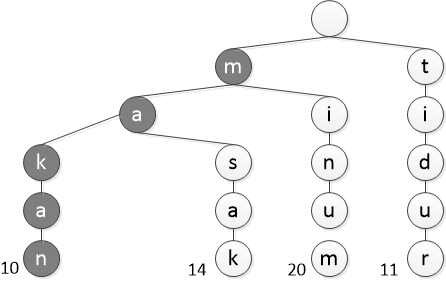
\includegraphics[width=\textwidth,keepaspectratio]{fig/TrieSearchingMakan.png}%
	\caption{Mencari kata $makan$ di Trie}%
	\label{fig:TrieSearchingMakan}%
\end{figure}

Pencarian \textit{node} akan berakhir apabila tidak ada \textit{node} yang cocok dengan kata pencarian kita, atau menemukan kata yang kita cari. Akan tetapi, walaupun kita sudah menemukan kata yang dicari, apabila tidak ada nilai dalam \textit{node} tersebut maka itu akan dianggap tidak ketemu. 

Contohnya jika kita mencari kata $maka$, akan ditemukan di jalur $makan$ tetapi tidak ada ditemukan nilai (null) di akhir pencarian maka kata $maka$ akan dianggap tidak ada di dalam $trie$.

\begin{figure}
    \includegraphics[width=\textwidth,keepaspectratio]{fig/TrieSearchingMaka.png}%
	\caption{Kata $maka$ ditemukan tetapi tidak memiliki nilai (bernilai null).}%
	\label{fig:TrieSearchingMaka}%
\end{figure}

Contoh lain, jika kita mencari kata $makin$, maka kita akan berhenti di huruf $k$ dan tidak bisa meneruskan lagi sehingga dianggap kata $makin$ tidak terdapat di trie.

\begin{figure}
    \includegraphics[width=\textwidth,keepaspectratio]{fig/TrieSearchingMakin.png}%
	\caption{Pencarian berhenti di huruf $k$ dan tidak bisa diteruskan sehingga kata $makin$ tidak ditemukan di trie.}%
	\label{fig:TrieSearchingMakin}%
\end{figure}

Pembentukan \textit{trie} dilakukan dengan menambahkan setiap string ke \textit{trie} dengan langkah berikut.
\begin{enumerate}
	\item Menggunakan karakter pertama dari string sebagai panduan untuk memasukkan ke \textit{trie}. Jika karakter sudah ada di \textit{trie} berupa \textit{node} maka gunakan \textit{node} tersebut untuk merepresentasikan karakter tersebut. Lanjutkan dengan karakter selanjutnya dari string.
	\item Jika tidak ada karakter yang ingin kita masukkan di \textit{trie} maka bentuk node baru.
	\item Apabila semua karakter sudah dimasukkan ke trie, masukkan nilai (\textit{value}) dari string ke karakter terakhir.
\end{enumerate}

Sebagai contoh, kita akan membentuk sebuah \textit{trie} dengan menggunakan string berikut: $she, sells, sea, shells, by, the, sea, shore$.

\begin{enumerate}
	\item Pertama masukkan string $she$. Karena belum ada \textit{node} dengan karakter awal $s$ maka, kita akan bentuk \textit{node} baru untuk semua string $she$. Kemudian berikan nilai 0 di akhir string $she$.
		\begin{figure}
			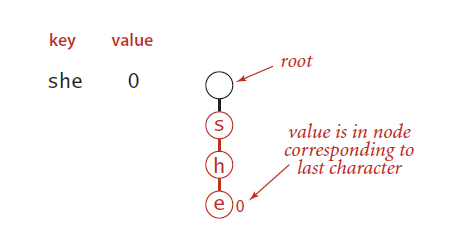
\includegraphics[width=\textwidth,keepaspectratio]{fig/FormTrie1.png}%
			\caption{String $she$ dimasukkan ke dalam Trie.}%
			\label{fig:FormTrie1}%
		\end{figure}
	\item Setelah string $she$, maka selanjutnya adalah string $sells$. Dalam memasukkan string $sells$, karakter pertama yaitu $s$ sudah dimasukkan, untuk itu \textit{node} untuk $s$ yang digunakan oleh $she$ juga digunakan untuk $sells$. Akan tetapi, karakter selanjutnya yaitu $e$ tidak ada setelah $s$ maka itu dibentuk node baru untuk $e$. Kemudian berikan nilai 1 di akhir $sells$.
		\begin{figure}
			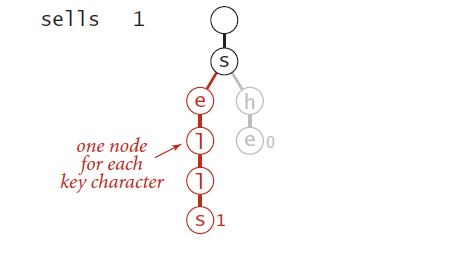
\includegraphics[width=\textwidth,keepaspectratio]{fig/FormTrie2.png}%
			\caption{String $sells$ dimasukkan ke dalam Trie.}%
			\label{fig:FormTrie2}%
		\end{figure}
	\item Lakukan hal yang sama untuk semua string yang tersisa.
		\begin{figure}
			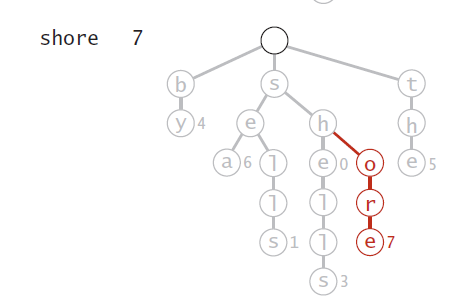
\includegraphics[width=\textwidth,keepaspectratio]{fig/FormTrie3.png}%
			\caption{Semua string dimasukkan ke dalam Trie.}%
			\label{fig:FormTrie3}%
		\end{figure}
\end{enumerate}

\subsection{Implementasi Python}

Untuk implementasi di python, akan menggunakan \textit{dictionary} sebagai dasar dari \textit{Trie}. Kita akan membuat sebuah \textit{class} \textit{Trie} yang terdapat beberapa metode seperti penambahan, penghapusan, dan sebagainya.

Kita akan melihat inisialisasi dari kelas \textit{Trie} yang dapat dilihat di Algoritma ~\ref{algo:trieinit}.
Dalam inisialisasi Trie tersebut variabel $path$ merupakan \textit{dictionary} yang akan menyimpan semua \textit{node} dari Trie. Sedangkan variabel $value$ akan menyimpan nilai dari \textit{node} tersebut. Variabel $value\_valid$ akan menyimpan data boolean yang menandakan apakah \textit{node} tersebut valid atau tidak.

\lstinputlisting[language=Python, 
                 firstline=1,
                 lastline=6,
                 label={algo:trieinit},
                 caption=Inisialisasi Kelas Trie
                ]
                {code/trie.py}
								
Untuk penambahan string baru bisa menggunakan metode di Algoritma ~\ref{algo:trieAdd}. 

\lstinputlisting[language=Python, 
                 firstline=8,
                 lastline=21,
                 label={algo:trieAdd},
                 caption=Penambahan String baru ke Trie
                ]
                {code/trie.py}

Dalam Algoritma ~\ref{algo:trieAdd}, pertama karakter awal dari string akan dimasukkan ke dalam variabel $head$. 

\lstinputlisting[language=Python, 
                 firstline=9,
                 lastline=9,        
                ]
                {code/trie.py}
								
Kemudian, kita akan mengecek apakah sebelumnya sudah ada karakter tersebut di dalam \textit{Trie}. Jika ada maka kita akan mulai dari \textit{node} yang berisikan karakter tersebut. Jika tidak, maka kita akan bentuk \textit{node} baru.

\lstinputlisting[language=Python, 
                 firstline=10,
                 lastline=14,        
                ]
                {code/trie.py}

Setelah itu kita cek apakah karakter yang kita masukkan merupakan yang terakhir dari string. Jika merupakan karakter terakhir maka kita akan akhiri dengan menset \textit{value} dari \textit{node} tersebut. Jika masih tersisa karakter lain, maka kita akan secara rekursif untuk memproses karakter lainnya.

\lstinputlisting[language=Python, 
                 firstline=16,
                 lastline=21,        
                ]
                {code/trie.py}

Untuk penghapusan, kita akan menggunakan metode di ~\ref{algo:trieremove}. 

\lstinputlisting[language=Python, 
                 firstline=23,
                 lastline=34,
                 label={algo:trieremove},
                 caption=Penghapusan node di Trie
                ]
                {code/trie.py}
								
Seperti penambahan, penghapusan string akan dimulai dengan pengecekan karakter pertama apakah ada di dalam \textit{trie} atau tidak.

\lstinputlisting[language=Python, 
                 firstline=24,
                 lastline=25,        
                ]
                {code/trie.py}

Jika ada dalam \textit{trie} maka, kita bisa menghapus string tersebut dengan menggunakan rekursif. 

\lstinputlisting[language=Python, 
                 firstline=26,
                 lastline=34,        
                ]
                {code/trie.py}

Untuk mengambil \textit{value} dari sebuah string, kita bisa menggunakan metode di ~\ref{algo:Trieget} dimana proses pengambilan \textit{value} dilakukan dengan rekursif sampai karakter terakhir untuk mengambil nilainya.

\lstinputlisting[language=Python, 
                 firstline=36,
                 lastline=51,
                 label={algo:Trieget},
                 caption=Mengambil \textit{value} node di Trie
                ]
                {code/trie.py}

Untuk mengecek apakah sebuah string ada atau tidak di dalam Trie bisa menggunakan metode di Algoritma ~\ref{algo:Triecontain}

\lstinputlisting[language=Python, 
                 firstline=36,
                 lastline=51,
                 label={algo:Triecontain},
                 caption=Mengecek apakah sebuah string ada atau tidak di Trie
                ]
                {code/trie.py}
								
Untuk mengambil semua string di Trie dengan prefix tertentu atau semuanya bisa menggunakan metode di Algoritma ~\ref{algo:Triekeys}.

\lstinputlisting[language=Python, 
                 firstline=36,
                 lastline=51,
                 label={algo:Triekeys},
                 caption=Mengambil semua string di Trie
                ]
                {code/trie.py}

\subsection{\textit{Suffix Trie}}

\textit{Suffix Trie} adalah sebuah \textit{Trie} biasa dimana isi dari \textit{Trie} tersebut adalah semua \textit{suffix} dari sebuah string. Sebagai contoh untuk string $abaaba$, maka kita bisa membentuk suffix berupa: $abaaba\$$, $baaba\$$, $aaba\$$, $aba\$$, $ba\$$, $a\$$, dan $\$$. Semua itu akan dibentuk sebuah \textit{trie} yang bisa dilihat di Gambar ~\ref{fig:suffixTrie}

	\begin{figure}
		\includegraphics[width=\textwidth,keepaspectratio]{fig/suffixTrie.png}%
		\caption{Sebuah \textit{suffix trie} dari string $abaaba$.}%
		\label{fig:suffixTrie}%
	\end{figure}

Implementasi dari \textit{Suffix Trie} sama seperti \textit{Trie} biasa hanya saja kita harus mencari dulu semua suffix dari sebuah string baru dimasukkan ke dalam \textit{Trie}. Untuk mencari semua suffix cukup iterasi dari awal string sampai akhir string dan potong satu karakter dari depan setiap kali iterasi.

Dengan menggunakan \textit{suffix trie}, banyak operasi pada string bisa dilakukan dengan cepat. \textit{Suffix trie} lebih efisien dalam penyimpanan dibandingkan dengan menyimpan dalam array biasa. Salah satu contoh pemanfaatan \textit{Suffix Trie} adalah mencari apakah sebuah substring merupakan bagian dari sebuah string misalnya: apakah substring $baa$ merupakan bagian dari $abaaba$? Untuk penyelesaiannya bisa dilihat di Gambar ~\ref{fig:suffixtriefindbaa}. Waktu yang diperlukan untuk mencari adalah sepanjang ukuran query atau O(|query|).

	\begin{figure}
		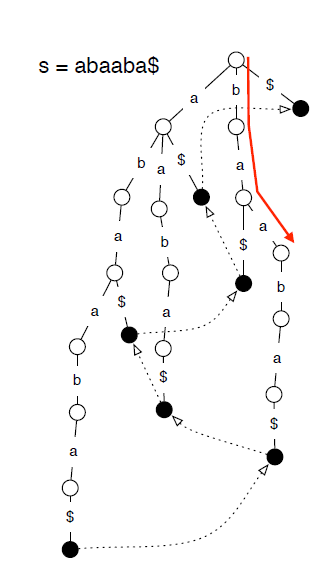
\includegraphics[width=\textwidth,keepaspectratio]{fig/suffixtriefindbaa.png}%
		\caption{Mencari substring $baa$ di string $abaaba$.}%
		\label{fig:suffixtriefindbaa}%
	\end{figure}

Ada banyak apalikasi lain untuk \textit{suffix trie} seperti:
\begin{enumerate}
	\item Mencari apakah sebuah string merupakan suffix dari string lain.
	\item Mencari \# kemunculan dari sebuah string dalam string lain.
	\item Mencari jumlah substring yang paling banyak muncul di sebuah string.
\end{enumerate}

\subsection{\textit{Suffix Tree}}

\textit{Suffix Tree} adalah pengembangan dari \textit{Suffix Trie} dimana semua \textit{node} yang tidak memiliki cabang dikompress menjadi satu \textit{node}. Lihat Gambar ~\ref{fig:suffixtree} untuk melihat \textit{suffix tree} dari string $abaaba$.

	\begin{figure}
		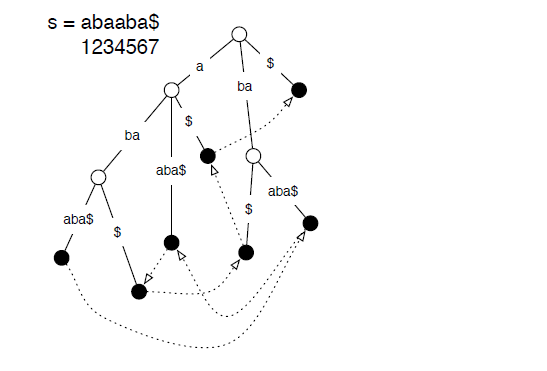
\includegraphics[width=\textwidth,keepaspectratio]{fig/suffixtree.png}%
		\caption{Suffix tree dari string $abaaba$. Perhatikan bahwa pohon menjadi lebih kecil dan lebih ruang efisien}%
		\label{fig:suffixtree}%
	\end{figure}
	
\subsection{\textit{Suffix Array}}

\textit{Suffix Array} merupakan \textit{Suffix Tree} yang disimpan di dalam sebuah array. Semua suffix dari sebuah string disimpan dalam array. Posisi setiap suffix dalam array sesuai dengan urutan \textit{lexicographic} (diurut berdasarkan alphabet setelah diurut berdasarkan panjang suffix). Lihat Gambar ~\ref{fig:suffixarray} untuk melihat \textit{Suffix Array} dari string $abaaba$.

	\begin{figure}
		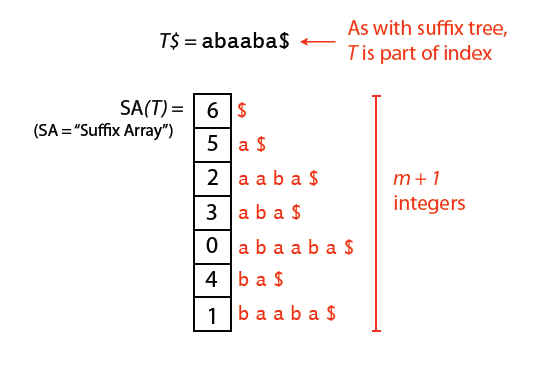
\includegraphics[width=\textwidth,keepaspectratio]{fig/suffixarray.png}%
		\caption{Suffix array dari string $abaaba$.}%
		\label{fig:suffixarray}%
	\end{figure}
	
Implementasi \textit{Suffix Array} adalah yang termudah dari semua. Lihat Algoritma ~\ref{algo:SuffixArray} untuk implementasi \textit{suffix array}.

\lstinputlisting[language=Python, 
                 firstline=4,
                 lastline=9,
                 label={algo:SuffixArray},
                 caption=Membentuk suffix array
                ]
                {code/suffixArray.py}

Untuk \textit{Suffix Array}, kita akan menggunakan \textit{OrderedDict} yang merupakan bagian dari \textit{collections}. Dengan \textit{dictionary} biasa kita tidak bisa mengurut isi dari \textit{dictionary}, akan tetapi dengan \textit{OrderedDict} kita bisa mengurut berdasarkan kunci. 

\section{Algoritma Pemrosesan String}

Untuk pemrosesan String terdapat banyak algoritma, kita akan melihat beberapa contoh algoritma yang bisa memanfaatkan \textit{suffix array}. Kita memilih menggunakan \textit{suffix array} dikarenakan implementasi \textit{suffix array} adalah yang paling mudah dibandingkan dengan \textit{suffix trie} dan \textit{suffix tree}.

\subsection{Pencarian \textit{pattern} Substring dalam String (\textit{String Matching})}

Dengan menggunakan \textit{Suffix Array} dari string $T$, kita bisa mencari \textit{pattern} string $P$ (dengan panjang $m$) dari string $T$ (panjang $n$) tersebut. Pencarian dengan menggunakan \textit{suffix array} lebih mudah dikarenakan 2 hal berikut.

\begin{enumerate}
	\item Jika seandainya $P$ adalah substring dari $T$, maka $P$ harus merupakan \textit{prefix} dari salah satu {suffix} $T$. 
	\item Karena dalam \textit{suffix array}, semua \textit{suffix} sudah diurut berdasarkan \textit{lexicography} maka pencarian \textit{prefix} lebih sederhana. Kita cukup mencocokkan setiap huruf dari urutan pertama dalam \textit{suffix array} sampai urutan terakhir secara berturut. 
\end{enumerate}

Cara naif untuk mencari \textit{pattern} substring dalam sebuah string dalam \textit{suffix array} adalah menggunakan pencarian sekuensial untuk mencocokkan \textit{prefix} dari semua \textit{suffix} yang ada dalam \textit{suffix array}. Untuk illustrasi bisa dilihat di Gambar ~\ref{fig:searchABSuffixArraySequential}.

	\begin{figure}
		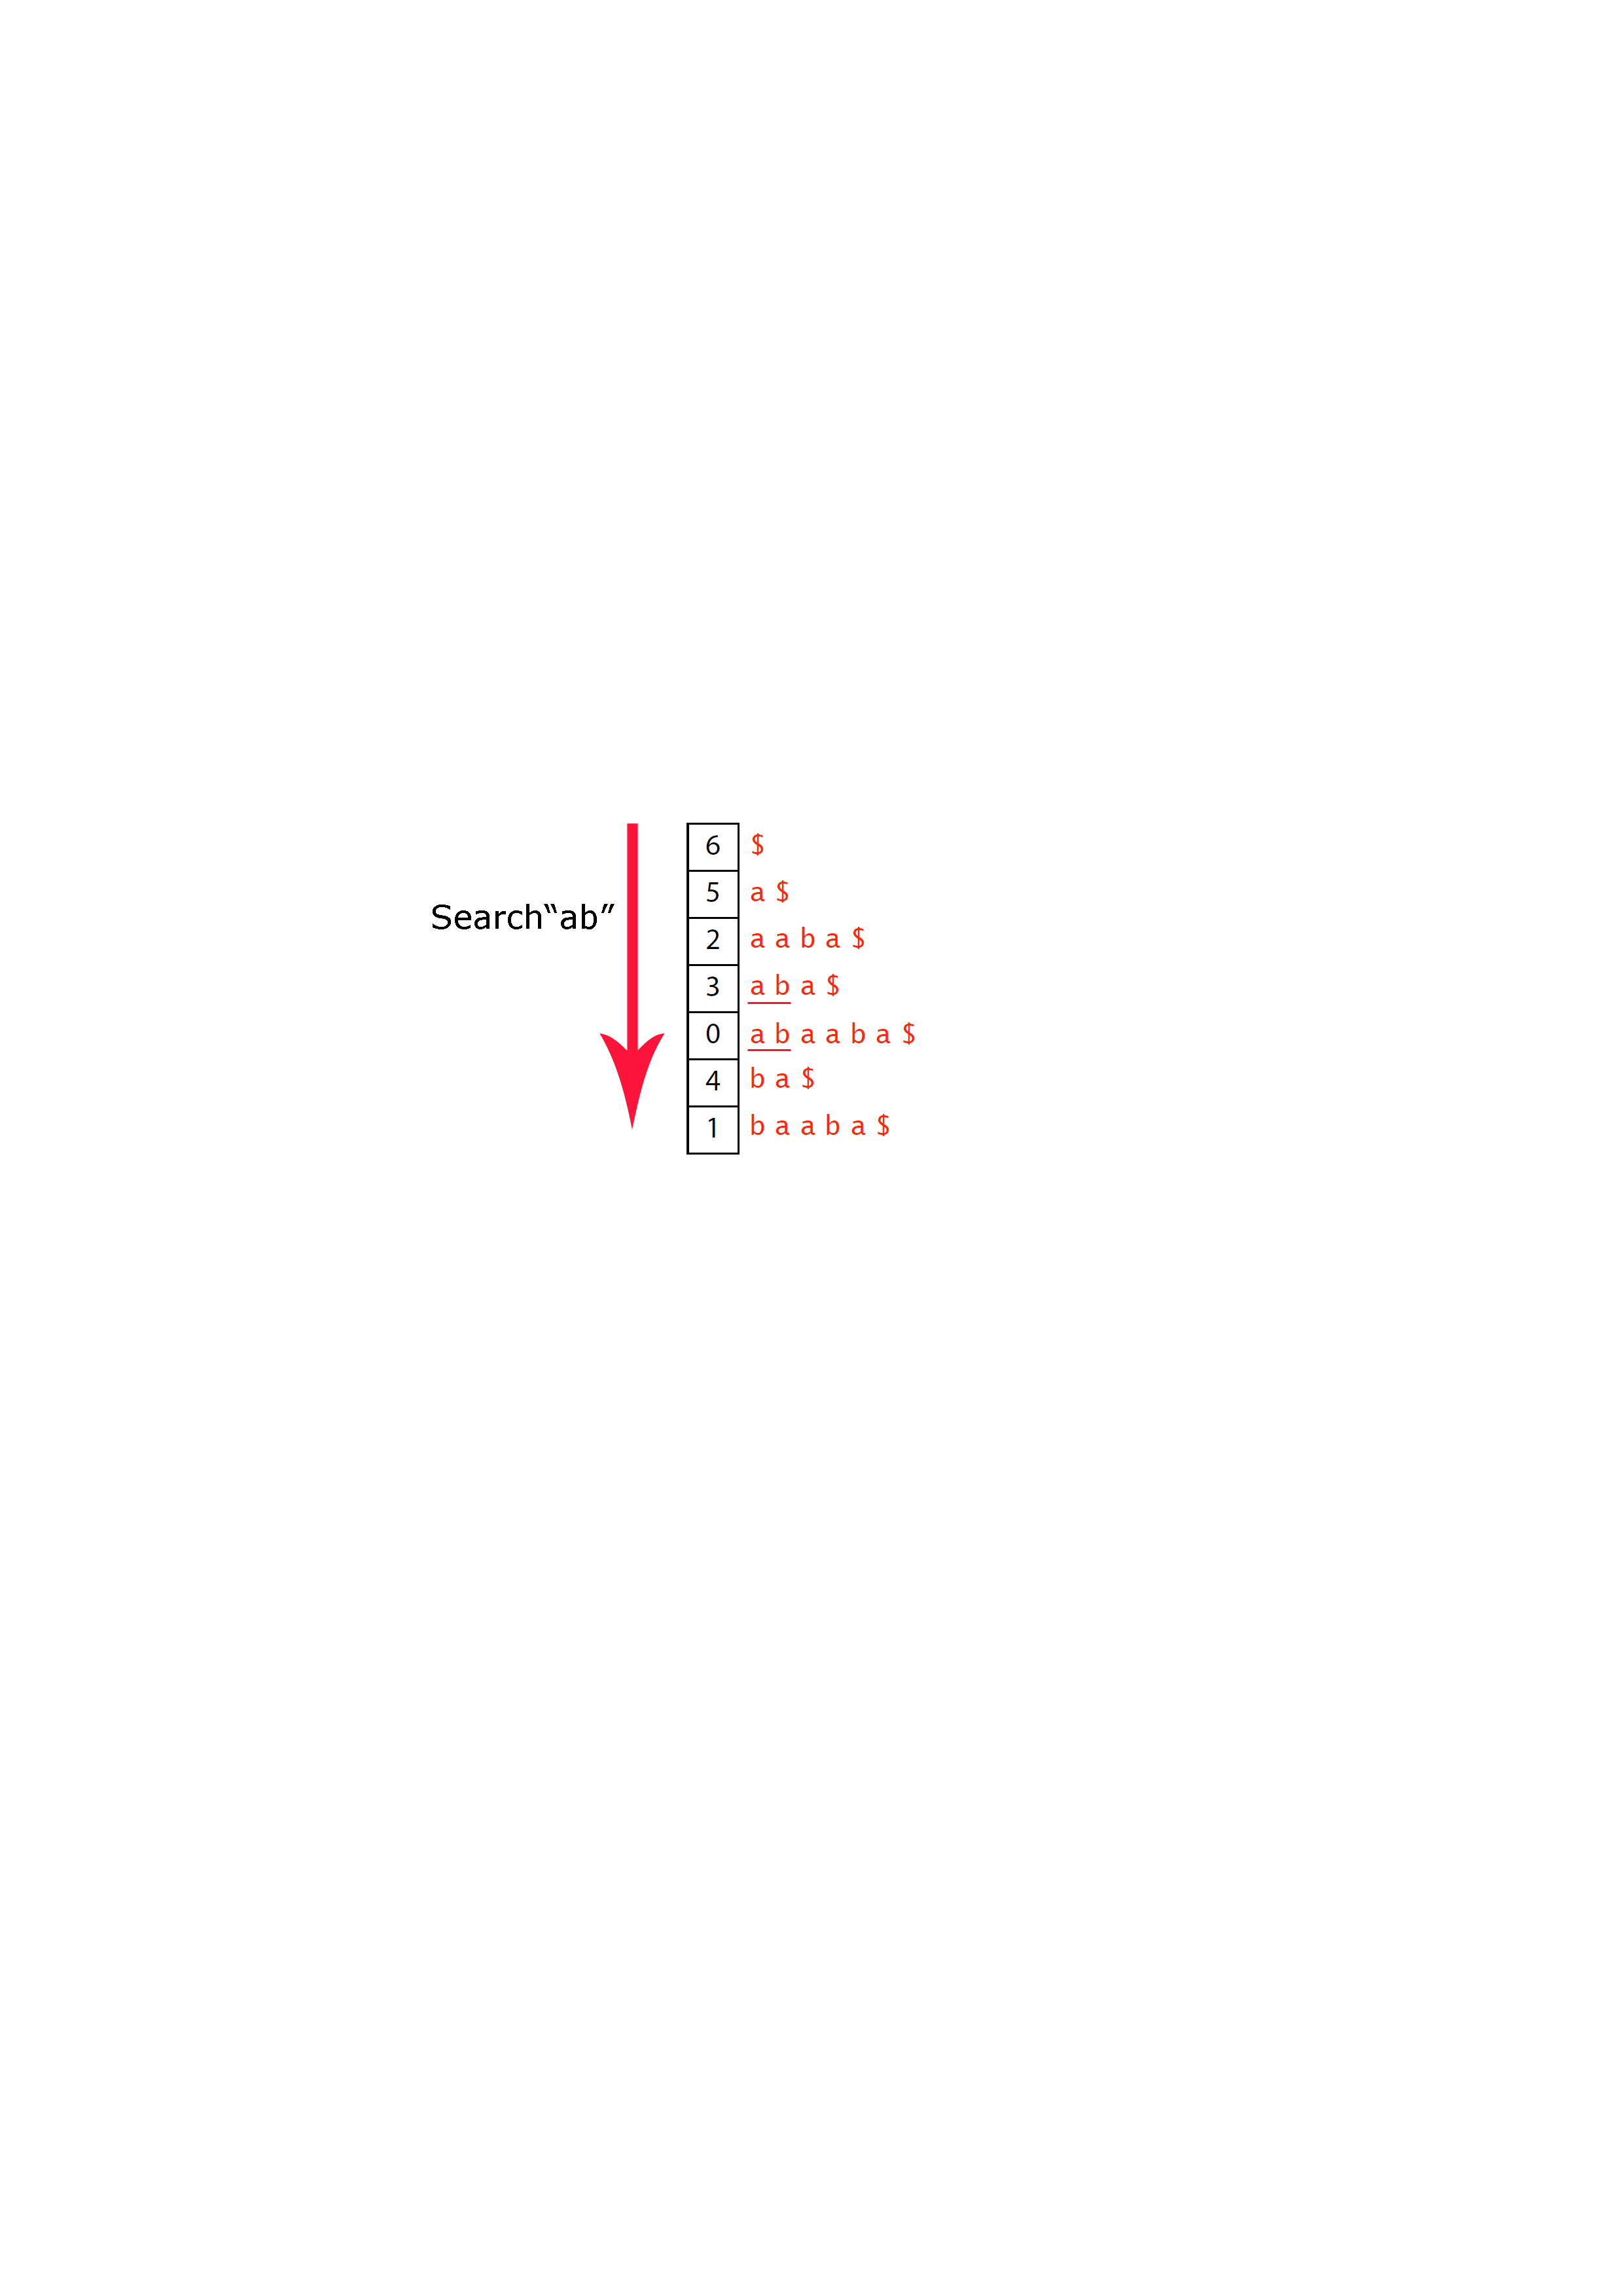
\includegraphics{fig/searchABSuffixArraySequential.png}%
		\caption{Mencari \textit{pattern} $ab$ dari string $abaaba$}%
		\label{fig:searchABSuffixArraySequential}%
	\end{figure}

Untuk implementasi pada Python bisa dilihat di Algoritma ~\ref{algo:StringMatchingNaif}.

\lstinputlisting[language=Python, 
                 firstline=11,
                 lastline=16,
                 label={algo:StringMatchingNaif},
                 caption=\textit{String Matching} naif dengan suffix array
                ]
                {code/suffixArray.py}


Untuk mempercepat pencarian, daripada menggunakan pencarian sekuensial kita akan menggunakan dua kali \textit{Binary Search} untuk mencari di bagian batas bawah dan batas atas. Waktu yang dibutuhkan untuk mencari adalah $O(m log n)$. Implementasi dari penggunaan \textit{Binary Search} bisa dilihat di Algoritma ~\ref{algo:StringMatchingBS}. 

\lstinputlisting[language=Python, 
                 firstline=18,
                 lastline=47,
                 label={algo:StringMatchingBS},
                 caption=\textit{String Matching} suffix array dengan Binary Search
                ]
                {code/suffixArray.py}

Cara kerja dari Algoritma ~\ref{algo:StringMatchingBS} bisa dilihat dari Gambar \ref{fig:StringMatchingBS} dimana kita akan mencari substring $GA$ dalama $GATAGACA$.

	\begin{figure}
		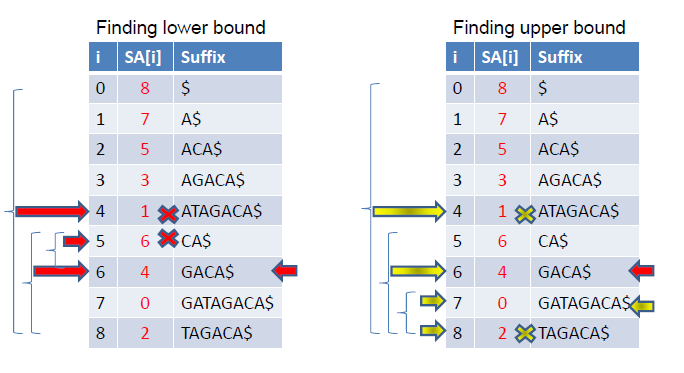
\includegraphics[width=\textwidth,keepaspectratio]{fig/StringMatchingBS.png}%
		\caption{\textit{String matching} dengan \textit{Binary Search}.}%
		\label{fig:StringMatchingBS}%
	\end{figure}
	
Perlu diketahui, bahwa berbeda dengan menggunakan pencarian sekuensial, kita tak perlu mencocokkan satu per satu setiap suffix dalam string $GATAGACA$. Melainkan kita hanya perlu mencari suffix pertama dan suffix terakhir dari string tersebut yang memuat substring $GA$. Sebagai contohnya, dari gambar kita mendapatkan suffix pertama yang memuat $GA$ adalah suffix posisi ke 6 (i=6) yaitu $GATAGACA$, dan suffix terakhir adalah suffix posisi ke 7 (i=7) yaitu $GACA$, maka secara otomatis semua suffix dalam posisi ke 6 dan ke 7 adalah suffix yang memuat $GA$ (karena posisi berdekatan maka hanya ada dua, coba lakukan sekali lagi dengan pencarian substring $A$).

Untuk mencari suffix pertama dan terakhir dibutuhkan dua kali \textit{Binary Search}. Satu untuk mencari yang pertama (\textit{lower bound}) dan satu lagi untuk mencari yang terakhir (\textit{upper bound}).

Untuk mencari suffix pertama kita akan menggunakan \textit{Binary Search} yang bisa dilihat di Algoritma ~\ref{algo:StringMatchingBS1}.

\lstinputlisting[language=Python, 
                 firstline=21,
                 lastline=29,
                 label={algo:StringMatchingBS1},
                 caption=\textit{Binary Search I} untuk mencari suffix pertama yang memuat substring
                ]
                {code/suffixArray.py}

Setelah kita menggunakan \textit{Binary Search} untuk mencari suffix pertama, kita akan mengecek apakah di posisi tersebut ada terdapat substring yang kita inginkan tidak. Jika tidak kita akan mengembalikan -1. Untuk pengecekan lihat di Algoritma ~\ref{algo:StringMatchingNF} 

\lstinputlisting[language=Python, 
                 firstline=30,
                 lastline=31,
                 label={algo:StringMatchingNF},
                 caption=Mengecek apakah di posisi tersebut terdapat substring yang kita inginkan atau tidak.
                ]
                {code/suffixArray.py}

Untuk mencari suffix kedua kita juga akan menggunakan \textit{Binary Search} yang bisa dilihat di Algoritma ~\ref{algo:StringMatchingBS2}.

\lstinputlisting[language=Python, 
                 firstline=21,
                 lastline=29,
                 label={algo:StringMatchingBS2},
                 caption=\textit{Binary Search II} untuk mencari suffix kedua yang memuat substring
                ]
                {code/suffixArray.py}



\subsection{Pencarian pattern terpanjang yang berulang di dalam string}

Diberikan sebuah string $T$, kita ingin mencari pattern $P$ terpanjang yang berulang (minimal >1) dalam string $T$. Misalnya: dalam string $banana$, maka pattern terpanjang yang berulang adalah $ana$.

Untuk menyelesaikan masalah tersebut, kita memerlukan sebuah struktur data yang lebih efisien dan merupakan pengembangan dari \textit{suffix array} yaitu \textit{longest common prefix suffix array} (LCPA. Dalam LCPA, semua panjang LCP akan dihitung dan disimpan dalam \textit{suffix array}. Definisi dari LCP adalah: ``Diberikan dua buah string yaitu $u$ dan $v$, maka prefix terpanjang yang terdapat di kedua buah string tersebut adalah LCP''. Sebagai contohnya:

LCP dari string $\textbf{a}$ dan $\textbf{a}abba$ adalah $a$ dengan panjang 1.

LCP dari string $\textbf{ab}aaabba$ dan $\textbf{ab}ba$ adalah $ab$ dengan panjang 2.

Sebagai contoh dari LCPA, kita bisa melihat contoh berikut dari string $banana$.


\begin{center}
  \begin{tabular}{ | c | c | c |c | c | c | c | c | }
    \hline
    i	& 1	& 2	& 3	& 4	& 5	& 6	& 7 \\ \hline
		A[i]	& 7	& 6	& 4	& 2	& 1	& 5	& 3 \\ \hline
		H[i]	& null	& 0 & 1 &	3 & 0 & 0 & 2 \\ \hline
		1	& \$	& a	& a	& a	& b	& n	& n \\ \hline
		2	& & \$	& n	& n	& a	& a	& a \\ \hline
		3	& & & a	& a	& n	& \$	& n \\ \hline
		4	& & & \$	& n	& a	& & a \\ \hline
		5 & & & & a	& n	& & \$ \\ \hline
		6	& & & & \$ & a	& & \\ \hline
		7	& & & & & \$ & &  \\ 
    \hline
  \end{tabular}
\end{center}

Dari tabel, H[i] merupakan LCP dari setiap suffix $banana$ yang ada. Cara membaca tabel adalah kita membanding setiap H[i] dengan H[i-1] dan mencari jumlah prefix terpanjang. Sebagai contohnya H[3] adalah 1 karena H[2] ($a\$$) dan H[3]($ana\$$) ada kesamaan prefix dengan panjang sebanyak 1 ($a$). Sedangkan H[4] adalah 3 karena H[4] ($anana\$$) dan H[3] ($ana\$$) memiliki kesamaan prefix dengan panjang sebanyak 3 ($ana$). Dengan menyusun LCPA dari setiap suffix, kita bisa mendapatkan prefix dengan jumlah karakter terpanjang sebanyak 3 yang berada di suffix ($anana\$$).

Algoritma pembentukan LCPA bisa dilihat di ~\ref{algo:LCPA}. Algoritma tersebut membentuk LCPA dengan menghitung prefix yang sama dari setiap suffix.

\lstinputlisting[language=Python, 
                 firstline=49,
                 lastline=58,
                 label={algo:LCPA},
                 caption=Pembentukan LCPA dari \textit{suffix array}
                ]
                {code/suffixArray.py}
